\documentclass[a4paper]{article}
\usepackage[14pt]{extsizes} 
\usepackage[utf8]{inputenc}
\usepackage[english, russian]{babel}
\usepackage{amsmath}
\usepackage{amsfonts}
\usepackage{amssymb}
\usepackage{graphicx}
\usepackage{indentfirst}
\usepackage{mathtools}
\begin{document}
\begin{center}
\hfill \break
{\large МИНЕСТЕРСТВО НАУКИ ВЫСШЕГО ОБРАЗОВАНИЯ РОССИЙСКОЙ ФЕДЕРАЦИИ}\\
{\large Федеральное государственное бюджетное образовательное учереждение высшего образования}\\
\hfill \break
{\large \textbf{"КУБАНСКИЙ ГОСУДАРСТВЕННЫЙ УНИВЕРСИТЕТ"}} \\
\hfill \break
{\large \underline {Факультет}}\: Математики и Компьютерных Наук\\
{\large \underline {Направление }}\: Математики и Компьютерных Наук\\

\hfill \break
\hfill \break
\hfill \break
{\Large Лабораторная работа №2}\\
{\Large Вариант  №17}\\
\hfill \break \hfill \break
\hfill \break \hfill \break
Работу выполнил \underline{\hspace{7cm}} Батурин Н.Ю.\\
\hfill \break
Специальность \underline{02.03.01 математика и компьютерные науки } курс \underline{ 2}\\
\hfill \break
Специализация \underline{\hspace{11cm}}\\
\hfill \break
Преподаватель \underline{\hspace{6cm}} Виноградова К.Н.\\
\hfill \break
\hfill \break 
\hfill \break \hfill \break
Краснодар\\
2023
\end{center}
\thispagestyle{empty}
\newpage
\begin{center}
\tableofcontents
\end{center}
\newpage
\section{Задание №1} 
\subsection{Условие:}
В двумерном массиве А, состоящем из n*m целых чисел вычислить:\newline
• 	сумму элементов;\newline
• 	количество ненулевых элементов, расположенных по периметру матрицы;\newline
• 	среднее геометрическое чисел, состоящих из различных цифр.\newline
•   Для заданной матрицы А(n×m) и матрицы того же типа и размерности С(n×m) найти значение выражения B = 2*A − 3*С.\newline
\subsection{Код:}\scriptsize
\begin{verbatim}
#include <iostream>
#include <ctime>
using namespace std;
bool Check(int ch) {
    int dubl_ch = ch, kol_cifr = 0;
    while (dubl_ch) {
        kol_cifr += 1;
        dubl_ch /= 10;
    }
    int* mas = new int[kol_cifr];
    for (int i = kol_cifr - 1; i >= 0; i--) {
        mas[i] = ch % 10;
        ch /= 10;
    }
    if (kol_cifr <= 1) {
        delete[]mas;
        return false;
    }
    for (int i = 0; i < kol_cifr / 2; i++)
        for (int j = kol_cifr - 1; j >= kol_cifr / 2; j--)
            if (mas[i] == mas[j]) {
                delete[]mas;
                return false;
            }
    delete[]mas;
    return true;
}
int main() {
    srand(time(NULL));
    int n, m, kol = 0; long int summa = 0; float pw = 1, st_pow = 0;
    cout << "\nn: "; cin >> n;
    cout << "m: "; cin >> m;
    int** A = new int* [n], ** B = new int* [n], ** C = new int* [n];
    for (int i = 0; i < n; i++) {
        A[i] = new int[m];
        B[i] = new int[m];
        C[i] = new int[m];
    }
    cout << "A:\n";
    for (int i = 0; i < n; i++) {
        for (int j = 0; j < m; j++) {
            A[i][j] = rand() % 10;
            cout << A[i][j] << " ";
            C[i][j] = rand() % 10;
            summa += A[i][j];
        }
        cout << endl;
    }
    cout << "\nC:\n";
    for (int i = 0; i < n; i++) {
        for (int j = 0; j < m; j++) {
            cout << C[i][j] << " ";
            if ((i == 0 || i == n - 1 || j == 0 || j == m - 1) && A[i][j] != 0)
                kol++;
            if (Check(A[i][j])) {
                st_pow++;
                pw *= A[i][j];
            }
            B[i][j] = 2 * A[i][j] - 3 * C[i][j];
        }
        cout << endl;
    }
    cout << "\nСумма: " << summa
        << "\nКол-во ненулевых элементов по периметру: " << kol
        << "\nCреднее геометрическое чисел: " << pow(pw, 1 / st_pow)
        << "\nB:\n";
    for (int i = 0; i < n; i++) {
        for (int j = 0; j < m; j++) cout << B[i][j] << " ";
        cout << endl;
    }
    for (int i = 0; i < n; i++) {
        delete[]A[i];
        delete[]B[i];
        delete[]C[i];
    }
    delete[]A;
    delete[]B;
    delete[]C;
    return 0;
}
\end{verbatim}\normalsize
\subsection{Результат:}
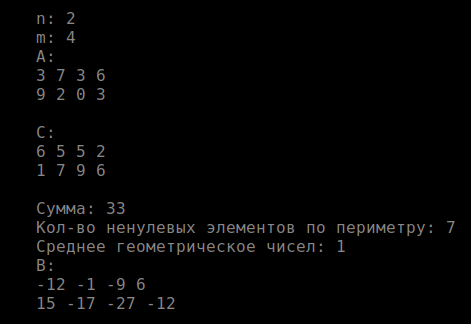
\includegraphics[width=1\textwidth]{1.png}
\newpage
\section{Задание №2} 
\subsection{Условие:}
Задана матрица целых чисел A(n×n). Сформировать массив B(n), каждый элемент которого равен количеству положительных элементов с чётной суммой цифр в  соответствующей строке матрицы. В столбцах матрицы поменять местами наибольший и наименьший элементы.
\subsection{Код:}\scriptsize
\begin{verbatim}
#include <iostream>
using namespace std;
bool Check_Chet(int ch) {
    int summa = 0;
    while (ch) {
        summa += ch % 10;
        ch /= 10;
    }
    if (summa % 2 == 0) return true;
    return false;
}
int main() {
    cout << "n: ";
    int n; cin >> n;
    int** A = new int* [n], * B = new int[n];
    for (int i = 0; i < n; i++) A[i] = new int[n];
    cout << "A:\n";
    for (int i = 0; i < n; i++) {
        for (int j = 0; j < n; j++)
            cin >> A[i][j];
        B[i] = 0;
    }
    for (int i = 0; i < n; i++)
        for (int j = 0; j < n; j++)
            if (Check_Chet(A[i][j]))B[i]++;
    for (int j = 0; j < n; j++) {
        int mx = A[0][j], mn = A[0][j], i1 = 0, i2 = 0, j1 = j, j2 = j;
        for (int i = 0; i < n; i++) {
            if (A[i][j] > mx) {
                mx = A[i][j];
                i1 = i;
                j1 = j;
            }
            if (A[i][j] < mn) {
                mn = A[i][j];
                i2 = i;
                j2 = j;
            }
        }
        swap(A[i1][j1], A[i2][j2]);
    }
    cout << "\nA:\n";
    for (int i = 0; i < n; i++) {
        for (int j = 0; j < n; j++) cout << A[i][j] << " ";
        cout << endl;
    }
    cout << "\nB: ";
    for (int i = 0; i < n; i++) cout << B[i] << " ";
    cout << endl;
    for (int i = 0; i < n; i++) delete[] A[i];
    delete[]A; delete[]B;
    return 0;
}
\end{verbatim}\normalsize
\subsection{Результат:}
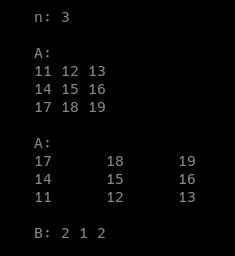
\includegraphics[width=0.9\textwidth]{2.png}
\newpage
\section{Задание №3} 
\subsection{Условие:}
Для матрицы I = 2*P -E, где Е — единичная матрица, а P=
\begin{pmatrix}
-26 & -18 & -27 \\
21 & 15 & 21 \\
12 & 8 & 13
\end{pmatrix}

При помощи метода Гаусса решить СЛАУ I*x = |1 1 1|^T.

Проверить свойство I^2 = E.
\subsection{Код:}\scriptsize
\begin{verbatim}
#include <iostream>
using namespace std;
bool Check(double** I, double** E) {
    double** I_pow_two = new double* [3];
    for (int i = 0; i < 3; i++) {
        I_pow_two[i] = new double[3];
        for (int j = 0; j < 3; j++) {
            I_pow_two[i][j] = 0;
            for (int k = 0; k < 3; k++)
                I_pow_two[i][j] += I[i][k] * I[k][j];
            if (I_pow_two[i][j] != E[i][j]) return false;
        }
    }
    return true;
}
double* Gauss(double** I, double* Units) {
    double* X, max;
    int k, index;
    const double eps = 0.00001;
    X = new double[3];
    k = 0;
    while (k < 3) {
        max = abs(I[k][k]);
        index = k;
        for (int i = k + 1; i < 3; i++) {
            if (abs(I[i][k]) > max) {
                max = abs(I[i][k]);
                index = i;
            }
        }
        for (int j = 0; j < 3; j++) {
            double temp = I[k][j];
            I[k][j] = I[index][j];
            I[index][j] = temp;
        }
        double temp = Units[k];
        Units[k] = Units[index];
        Units[index] = temp;
        for (int i = k; i < 3; i++) {
            double temp = I[i][k];
            if (abs(temp) < eps) continue;
            for (int j = 0; j < 3; j++)
                I[i][j] = I[i][j] / temp;
            Units[i] = Units[i] / temp;
            if (i == k)  continue;
            for (int j = 0; j < 3; j++)
                I[i][j] = I[i][j] - I[k][j];
            Units[i] = Units[i] - Units[k];
        }
        k++;
    }
    for (k = 2; k >= 0; k--) {
        X[k] = Units[k];
        for (int i = 0; i < k; i++)
            Units[i] = Units[i] - I[i][k] * X[k];
    }
    return X;
}
int main() {
    double** P = new double* [3], ** E = new double* [3], ** I = new double* [3], * Units = new double[3], * X;
    for (int i = 0; i < 3; i++) {
        P[i] = new double[3];
        E[i] = new double[3];
        I[i] = new double[3];
        Units[i] = 1;
        for (int j = 0; j < 3; j++)
            E[i][j] = 1;
    }
    P[0][0] = -26;
    P[0][1] = -18;
    P[0][2] = -27;
    P[1][0] = P[1][2] = 21;
    P[1][1] = 15;
    P[2][0] = 12;
    P[2][1] = 8;
    P[2][2] = 13;
    cout << "I:\n";
    for (int i = 0; i < 3; i++) {
        for (int j = 0; j < 3; j++) {
            I[i][j] = 2 * P[i][j] - E[i][j];
            cout << I[i][j] << " ";
        }
        cout << endl;
    }
    cout << "\nX:\n";
    X = Gauss(I, Units);
    for (int i = 0; i < 3; i++)
        cout << X[i] << " ";
    cout << endl;
    if (Check(I, E))cout << "\nПроверка пройдена успешно\n";
    else cout << "\nПроверка пройдена неудачно\n";
    cout << endl;
    return 0;
}
\end{verbatim}\normalsize
\subsection{Результат:}
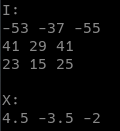
\includegraphics[width=1\textwidth]{3.png}
\newpage
\section{Задание №4} 
\subsection{Пункт №1}
\subsubsection{Условие:}
Реализовать классический алгоритм умножения квадратных матриц со всеми возможными перестановками порядка циклов (i,j,k) с использованием представления матриц в виде двумерных динамических массивов.
\subsubsection{Код:}\scriptsize
\begin{verbatim}
for (int i = 0; i < n; i++)
        for (int j = 0; j < n; j++) {
            C[i][j] = 0;
            for (int k = 0; k < n; k++)
                C[i][j] += A[i][k] * B[k][j];
        }
\end{verbatim}\normalsize
\subsection{Пункт №2}
\subsection{Условие:}
Провести тестирование программ классического умножения матриц (размерности 500, 1000, 2000). Внести в таблицу данные о времени выполнения программ (в секундах).
\subsubsection{Код:}\scriptsize
\begin{verbatim}
#include <iostream>
#include <string>
#include <ctime>
#include <chrono>
using namespace std;
using namespace std::chrono;
void multiplication_mat(int** A, int** B, int** C, int n, string choose) {
    if (choose == "IJK") {
        for (int i = 0; i < n; i++)
            for (int j = 0; j < n; j++) {
                C[i][j] = 0;
                for (int k = 0; k < n; k++)
                    C[i][j] += A[i][k] * B[k][j];
            }
    }
    if (choose == "IKJ") {
        for (int i = 0; i < n; i++)
            for (int k = 0; k < n; k++) {
                C[i][k] = 0;
                for (int j = 0; j < n; j++)
                    C[i][j] += A[i][k] * B[k][j];
            }
    }
    if (choose == "JIK") {
        for (int j = 0; j < n; j++)
            for (int i = 0; i < n; i++) {
                C[j][i] = 0;
                for (int k = 0; k < n; k++)
                    C[i][j] += A[i][k] * B[k][j];
            }
    }
    if (choose == "JKI") {
        for (int j = 0; j < n; j++)
            for (int k = 0; k < n; k++) {
                C[j][k] = 0;
                for (int i = 0; i < n; i++)
                    C[i][j] += A[i][k] * B[k][j];
            }
    }
    if (choose == "KIJ") {
        for (int k = 0; k < n; k++)
            for (int i = 0; i < n; i++) {
                C[k][i] = 0;
                for (int j = 0; j < n; j++)
                    C[i][j] += A[i][k] * B[k][j];
            }
    }
    if (choose == "KJI") {
        for (int k = 0; k < n; k++)
            for (int j = 0; j < n; j++) {
                C[k][j] = 0;
                for (int i = 0; i < n; i++)
                    C[i][j] += A[i][k] * B[k][j];
            }
    }
}
int main() {
    setlocale(LC_ALL, "Rus");
    cout << "Размер матриц:\tIJK\tIKJ\tJIK\tJKI\tKIJ\tKJI\n";
    srand(time(NULL));
    int size_matr = 0;
    while (size_matr < 2000) {
        size_matr += 500;
        cout << size_matr << "\t\t";
        int** Matr1 = new int* [size_matr], ** Matr2 = new int* [size_matr], ** C = new int* [size_matr];
        for (int i = 0; i < size_matr; i++) {
            Matr1[i] = new int[size_matr];
            Matr2[i] = new int[size_matr];
            C[i] = new int[size_matr];
        }
        for (int i = 0; i < size_matr; i++)
            for (int j = 0; j < size_matr; j++) {
                Matr1[i][j] = rand() % 1000;
                Matr2[i][j] = rand() % 1000;
            }
        auto timeNULL = high_resolution_clock::now();
        multiplication_mat(Matr1, Matr2, C, size_matr, "IJK");
        auto timeONE = high_resolution_clock::now();
        cout << duration_cast<milliseconds>(timeONE - timeNULL).count() / 1000 << "\t";
        timeNULL = high_resolution_clock::now();
        multiplication_mat(Matr1, Matr2, C, size_matr, "IKJ");
        timeONE = high_resolution_clock::now();
        cout << duration_cast<milliseconds>(timeONE - timeNULL).count() / 1000 << "\t";
        timeNULL = high_resolution_clock::now();
        multiplication_mat(Matr1, Matr2, C, size_matr, "JIK");
        timeONE = high_resolution_clock::now();
        cout << duration_cast<milliseconds>(timeONE - timeNULL).count() / 1000 << "\t";
        timeNULL = high_resolution_clock::now();
        multiplication_mat(Matr1, Matr2, C, size_matr, "JKI");
        timeONE = high_resolution_clock::now();
        cout << duration_cast<milliseconds>(timeONE - timeNULL).count() / 1000 << "\t";
        timeNULL = high_resolution_clock::now();
        multiplication_mat(Matr1, Matr2, C, size_matr, "KIJ");
        timeONE = high_resolution_clock::now();
        cout << duration_cast<milliseconds>(timeONE - timeNULL).count() / 1000 << "\t";
        timeNULL = high_resolution_clock::now();
        multiplication_mat(Matr1, Matr2, C, size_matr, "KJI");
        timeONE = high_resolution_clock::now();
        cout << duration_cast<milliseconds>(timeONE - timeNULL).count() / 1000 << "\n";
        for (int i = 0; i < size_matr; i++) {
            delete[]Matr1[i];
            delete[]Matr2[i];
            delete[]C[i];
        }
        delete[]Matr1; delete[]Matr2; delete[]C;
    }
    return 0;
}
\end{verbatim}\normalsize
\subsubsection{Результат:}
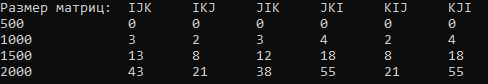
\includegraphics[width=1\textwidth]{4_2.png}
\subsection{Пункт №3}
\subsubsection{Условие:}
Выполнить 1-2 на матрицах представленных в виде одномерных массивов
\subsubsection{Код:}\scriptsize
\begin{verbatim}
#include <iostream>
#include <ctime>
#include <chrono>
using namespace std;
using namespace std::chrono;
void multiplication_mas(int* A, int* B, int* C, int size1, int size2, string choose) {
    if (choose == "IJK")
        for (int i = 0; i < size1; i++)
            for (int j = 0; j < size1; j++) {
                B[i * size1 + j] = 0;
                for (int k = 0; k < size1; k++)
                    B[i * size1 + j] += A[i * size1 + k]
                    * C[k * size1 + j];
            }
    if (choose == "IKJ")
        for (int i = 0; i < size1; i++)
            for (int k = 0; k < size1; k++) {
                B[i * size1 + k] = 0;
                for (int j = 0; j < size1; j++)
                    B[i * size1 + j] += A[i * size1 + k]
                    * C[k * size1 + j];
            }
    if (choose == "JIK")
        for (int j = 0; j < size1; j++)
            for (int i = 0; i < size1; i++) {
                B[j * size1 + i] = 0;
                for (int k = 0; k < size1; k++)
                    B[i * size1 + j] += A[i * size1 + k]
                    * C[k * size1 + j];
            }
    if (choose == "JKI")
        for (int j = 0; j < size1; j++)
            for (int k = 0; k < size1; k++) {
                B[j * size1 + k] = 0;
                for (int i = 0; i < size1; i++)
                    B[i * size1 + j] += A[i * size1 + k]
                    * C[k * size1 + j];
            }
    if (choose == "KIJ")
        for (int k = 0; k < size1; k++)
            for (int i = 0; i < size1; i++) {
                B[k * size1 + i] = 0;
                for (int j = 0; j < size1; j++)
                    B[i * size1 + j] += A[i * size1 + k]
                    * C[k * size1 + j];
            }
    if (choose == "KJI")
        for (int k = 0; k < size1; k++)
            for (int j = 0; j < size1; j++) {
                B[k * size1 + j] = 0;
                for (int i = 0; i < size1; i++)
                    B[i * size1 + j] += A[i * size1 + k]
                    * C[k * size1 + j];
            }
}
int main() {
    srand(time(NULL));
    cout << "\n\tРазмер массива:\tIJK\tIKJ\tJIK\tJKI\tKIJ\tKJI\n";
    int size1 = 0;
    while (size1 < 2000) {
        size1 += 500;
        cout << "\t" << size1 << " * " << size1 << "\t";
        int size2 = size1 * size1, * mas_A = new int[size2], * mas_C = new int[size2], * mas_B = new int[size2];
        for (int i = 0; i < size2; i++) {
            mas_A[i] = rand() % 100;
            mas_C[i] = rand() % 100;
        }
        auto timeNULL = high_resolution_clock::now();
        multiplication_mas(mas_A, mas_B, mas_C, size1, size2, "IJK");
        auto timeONE = high_resolution_clock::now();
        cout << duration_cast<milliseconds>(timeONE - timeNULL).count() / 1000 << "\t";
        timeNULL = high_resolution_clock::now();
        multiplication_mas(mas_A, mas_B, mas_C, size1, size2, "IKJ");
        timeONE = high_resolution_clock::now();
        cout << duration_cast<milliseconds>(timeONE - timeNULL).count() / 1000 << "\t";
        timeNULL = high_resolution_clock::now();
        multiplication_mas(mas_A, mas_B, mas_C, size1, size2, "JIK");
        timeONE = high_resolution_clock::now();
        cout << duration_cast<milliseconds>(timeONE - timeNULL).count() / 1000 << "\t";
        timeNULL = high_resolution_clock::now();
        multiplication_mas(mas_A, mas_B, mas_C, size1, size2, "JKI");
        timeONE = high_resolution_clock::now();
        cout << duration_cast<milliseconds>(timeONE - timeNULL).count() / 1000 << "\t";
        timeNULL = high_resolution_clock::now();
        multiplication_mas(mas_A, mas_B, mas_C, size1, size2, "KIJ");
        timeONE = high_resolution_clock::now();
        cout << duration_cast<milliseconds>(timeONE - timeNULL).count() / 1000 << "\t";
        timeNULL = high_resolution_clock::now();
        multiplication_mas(mas_A, mas_B, mas_C, size1, size2, "KJI");
        timeONE = high_resolution_clock::now();
        cout << duration_cast<milliseconds>(timeONE - timeNULL).count() / 1000 << "\n";
        delete[]mas_A, delete[]mas_B, delete[]mas_C;
    }
    return 0;
}
\end{verbatim}\normalsize
\subsubsection{Результат:}
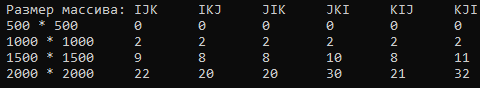
\includegraphics[width=1\textwidth]{4_3.png}
\end{document}